%%%%%%%%%%%%%%%%%%%%%%%%%%%%%%%%%%%%%%%%%
% Jacobs Landscape Poster
% LaTeX Template
% Version 1.1 (14/06/14)
%
% Created by:
% Computational Physics and Biophysics Group, Jacobs University
% https://teamwork.jacobs-university.de:8443/confluence/display/CoPandBiG/LaTeX+Poster
% 
% Further modified by:
% Nathaniel Johnston (nathaniel@njohnston.ca)
%
% This template has been downloaded from:
% http://www.LaTeXTemplates.com
%
% License:
% CC BY-NC-SA 3.0 (http://creativecommons.org/licenses/by-nc-sa/3.0/)
%
%%%%%%%%%%%%%%%%%%%%%%%%%%%%%%%%%%%%%%%%%

%----------------------------------------------------------------------------------------
%	PACKAGES AND OTHER DOCUMENT CONFIGURATIONS
%----------------------------------------------------------------------------------------

\documentclass[final]{beamer}

\usepackage[scale=1.0]{beamerposter} % Use the beamerposter package for laying out the poster
\usepackage{lmodern} 
\usepackage{amsmath}
\usepackage{amssymb}
\usepackage{bm}
\usepackage{subcaption}
\labelformat{subfigure}{}%() number
\usetheme{confposter} % Use the confposter theme supplied with this template
\usepackage{graphicx}
\usepackage{graphicx}  % Required for including images
\usepackage{tabularx}
\usepackage{booktabs} % Top and bottom rules for tables
\usepackage{tikz}
\usetikzlibrary{arrows.meta,
positioning,
quotes, shapes}

\usetikzlibrary{arrows}
\tikzset{
  double -latex/.style args={#1 colored by #2 and #3}{    
    -latex,line width=#1,#2,
    postaction={draw,-latex,#3,line width=(#1)/3,shorten <=(#1)/4,shorten >=4.5*(#1)/3},
  },
  double round cap-latex/.style args={#1 colored by #2 and #3}{    
    round cap-latex,line width=#1,#2,
    postaction={draw,round cap-latex,#3,line width=(#1)/3,shorten <=(#1)/4,shorten >=4.5*(#1)/3},
  },
  double round cap-stealth/.style args={#1 colored by #2 and #3}{
    round cap-stealth,line width=#1,#2,
    postaction={round cap-stealth,draw,,#3,line width=(#1)/3,shorten <=(#1)/3,shorten >=2*(#1)/3},
  },
  double -stealth/.style args={#1 colored by #2 and #3}{
    -stealth,line width=#1,#2,
    postaction={-stealth,draw,,#3,line width=(#1)/3,shorten <=(#1)/3,shorten >=2*(#1)/3},
  },
}
\usepackage[most]{tcolorbox}
\setbeamercolor{block title}{fg=dblue!80,bg=white} % Colors of the block titles
\setbeamercolor{block body}{fg=black,bg=white} % Colors of the body of blocks
\setbeamercolor{block alerted title}{fg=white,bg=dblue!70} % Colors of the highlighted block titles
\setbeamercolor{block alerted body}{fg=black,bg=dblue!10} % Colors of the body of highlighted blocks
% Many more colors are available for use in beamerthemeconfposter.sty
% declare `cmex` to be arbitrary scalable
\DeclareFontShape{OMX}{cmex}{m}{n}{
  <-7.5> cmex7
  <7.5-8.5> cmex8
  <8.5-9.5> cmex9
  <9.5-> cmex10
}{}

\SetSymbolFont{largesymbols}{normal}{OMX}{cmex}{m}{n}
\SetSymbolFont{largesymbols}{bold}  {OMX}{cmex}{m}{n}


%-----------------------------------------------------------
% Define the column widths and overall poster size
% To set effective sepwid, onecolwid and twocolwid values, first choose how many columns you want and how much separation you want between columns
% In this template, the separation width chosen is 0.024 of the paper width and a 4-column layout
% onecolwid should therefore be (1-(# of columns+1)*sepwid)/# of columns e.g. (1-(4+1)*0.024)/4 = 0.22
% onecolwid should therefore be (1-(# of columns+1)*sepwid)/# of columns e.g. 
% (1-(3+1)*0.025)/3 = 0.3
% Set twocolwid to be (2*onecolwid)+sepwid = 0.464
% Set threecolwid to be (3*onecolwid)+2*sepwid = 0.708

\newlength{\sepwid}
\newlength{\onecolwid}
\newlength{\twocolwid}
\newlength{\threecolwid}
\setlength{\paperwidth}{48in} % A0 width: 46.8in
\setlength{\paperheight}{32in} % A0 height: 33.1in
\setlength{\textwidth}{46in} % A0 width: 46.8in
\setlength{\textheight}{34in} % A0 height: 33.1in
\setlength{\sepwid}{0.025\paperwidth} % Separation width (white space) between columns
\setlength{\onecolwid}{0.3\paperwidth} % Width of one column
\setlength{\twocolwid}{0.625\paperwidth} % Width of two columns
\setlength{\threecolwid}{0.95\paperwidth} % Width of three columns
\setlength{\topmargin}{0.5in} % Reduce the top margin size
\setlength{\leftmargin}{0.5in} % Reduce the top margin size
%-----------------------------------------------------------









%----------------------------------------------------------------------------------------
%	TITLE SECTION 
%----------------------------------------------------------------------------------------

\title{%
  \texorpdfstring{%
    \makebox[\linewidth]{%
      \makebox[-200pt][l]{%
        \raisebox{\dimexpr-\height+\baselineskip}[0pt][0pt]
          {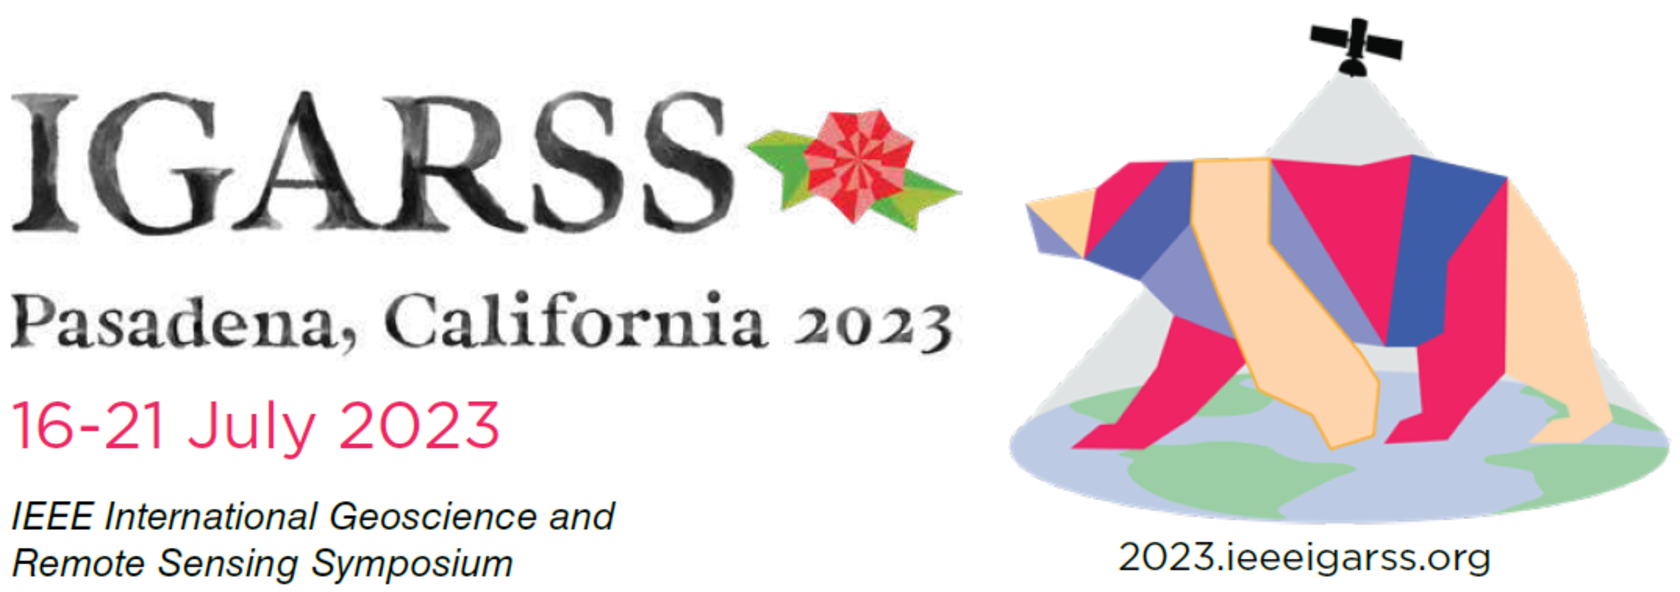
\includegraphics[height=2.7\baselineskip]{figures/logo_IG23.pdf}}}% Left logo
      \hfill
      \makebox[\dimexpr\linewidth-4em][c]{%
        \begin{minipage}{\linewidth}
          \centering
          \LARGE QUALITY ASSESSMENT MEASURES FOR EXPLAINABLE FUSION OF STATISTICAL\\ EVIDENCES OF EDGES IN POLSAR IMAGES: A FIRST APPROACH
        \end{minipage}
      }%
      \hfill\hspace{-50cm} %
      \raisebox{\dimexpr-\height-1.1\baselineskip}[0pt][0pt] % 
        {
\includegraphics[height=2.9\baselineskip]{../../Figures/PNG/QRCode-WebPageVUW.png}}% New figure
      \hfill
      \raisebox{\dimexpr-\height+\baselineskip}[0pt][0pt]
        {
\includegraphics[height=3.0\baselineskip]{figures/logos.pdf}}% Right logo
    }%
  }%
}

\author{\vspace*{2cm}Rosa Janeth Alpala$^1$,  Anderson A.\ de Borba$^{2,3}$  and \textbf{Alejandro C.\ Frery}$^3$}
\institute[]{%
  \makebox[\linewidth]{%
    \begin{minipage}[c]{0.6\linewidth}
      \centering
      \vspace{0.5cm}
      $^1$Universidade Federal de Pernambuco, Recife, Brazil\\
      $^2$Mackenzie Presbyterian University--UPM, FCI, BigMAAp, SP -- Brazil\\
      $^3$School of Mathematics and Statistics, Victoria University of Wellington, New Zealand
    \end{minipage}%
    
}}

%\title{%
  %\texorpdfstring{%
    %\makebox[\linewidth]{	%
      %\makebox[-100pt][l]{%
        %\raisebox{\dimexpr-\height+\baselineskip}[0pt][0pt]
          %{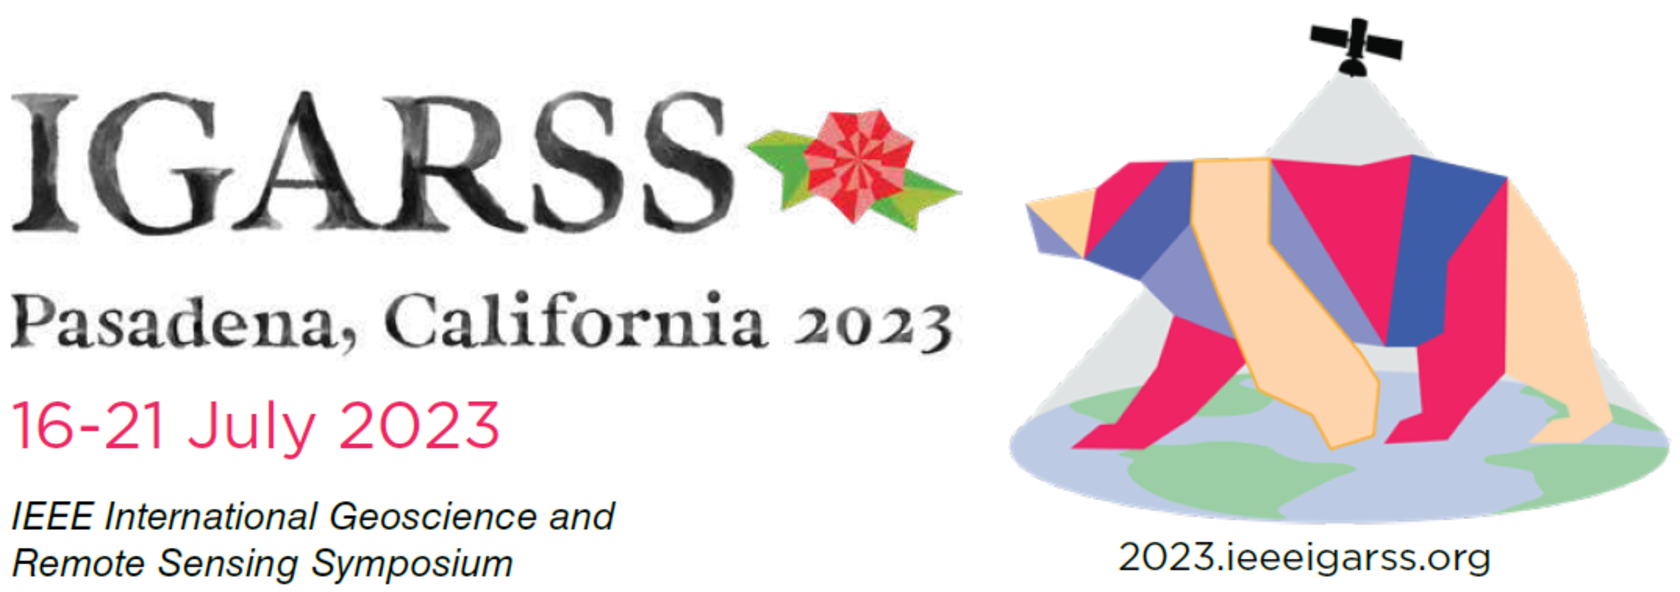
\includegraphics[height=2.7\baselineskip]{figures/logo_IG23.pdf}}% Left logo
      %}\hfill
			%\makebox[\dimexpr\linewidth-4em][c]{%
        %\begin{minipage}{\linewidth}
          %\centering
          %\LARGE QUALITY ASSESSMENT MEASURES FOR EXPLAINABLE FUSION OF STATISTICAL\\ EVIDENCES OF EDGES IN POLSAR IMAGES: A FIRST APPROACH
        %\end{minipage}
      %}%
      %\hfill\hspace{-20cm} % Ajusta la cantidad de espacio según tus necesidades
      %\raisebox{\dimexpr-\height-1.5\baselineskip}[0pt][0pt] % Ajusta la cantidad de espacio según tus necesidades
        %{
\includegraphics[height=2.7\baselineskip]{../../Figures/PNG/QRCode-WebPageVUW.png}}% New logo
            %\hfill\makebox[-50pt][r]{%
        %\raisebox{\dimexpr-\height+\baselineskip}[0pt][0pt]
          %{
\includegraphics[height=3.0\baselineskip]{figures/logos.pdf}}% Right logo
      %}%
    %}%
  %}
  %} % Poster title
	%
	%\author{\vspace*{2cm}Rosa Janeth Alpala$^1$,  Anderson A.\ de Borba$^{2,3}$  and \textbf{Alejandro C.\ Frery}$^3$}
%\institute[]{$^1$Universidade Federal de Pernambuco, Recife, Brazil\\
%$^2$Mackenzie Presbyterian University--UPM, FCI, BigMAAp, SP -- Brazil\\
%$^3$School of Mathematics and Statistics, Victoria University of Wellington, New Zealand}
	
%%----------------------------------------------------------------------------------------

\begin{document}



\setlength{\belowcaptionskip}{2ex} % White space under figures
\setlength\belowdisplayshortskip{2ex} % White space under equations

\begin{frame}[t] % The whole poster is enclosed in one beamer frame

\begin{columns}[t,totalwidth=\threecolwid] % The whole poster consists of three major columns

\begin{column}{0.5\sepwid}\end{column} % Empty spacer column

\begin{column}{\onecolwid} % 

%----------------------------------------------------------------------------------------
%	The first column
%----------------------------------------------------------------------------------------

\begin{block}{\LARGE{SETUP}}
\vspace{0.7em}
\begin{figure}[h]
  \centering
  \caption*{\large{Flevoland}}
  \vspace{-15pt}
  \begin{tikzpicture}%%[trim={left bottom right top},clip] reduce image borders
    \node (figure) at (0,0) {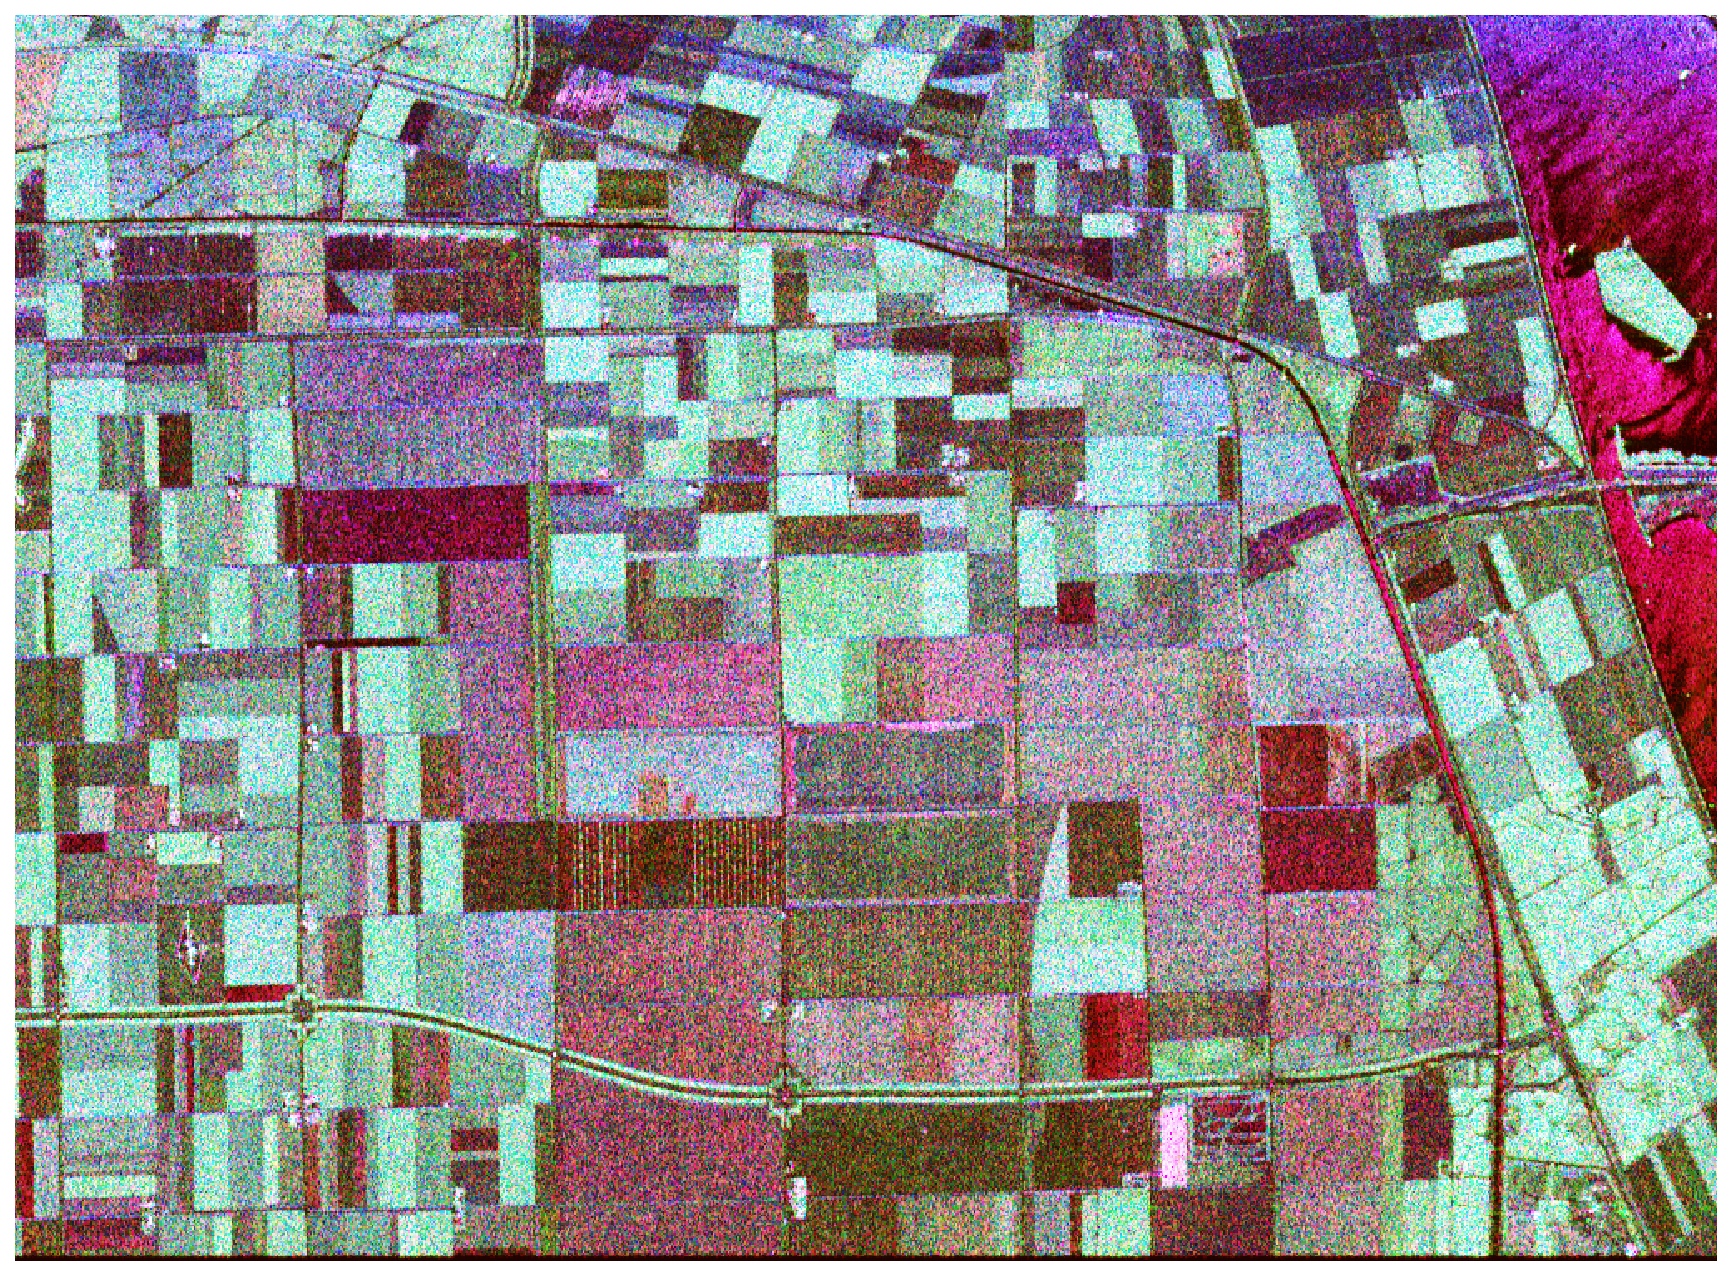
\includegraphics[trim={2cm 8cm 15cm 3cm},clip,width=25cm]{figures/flev_pauli_total.pdf}};
    \draw[double -stealth=10pt colored by blue!50!black and white] (figure.south) -- ++(0,-4cm);
    \node[below=of figure, yshift=-3cm] (text) {\begin{tcolorbox}[colback=blue!10,colframe=blue!30!black, arc=2pt, outer arc=2pt, nobeforeafter, width=7cm, center upper]
      \textbf{Edge Detection}
    \end{tcolorbox}};
    \node[below left=of text, xshift=-2.5cm] (text1) {\begin{tcolorbox}[colback=green!10,colframe=green!30!black, arc=2pt, outer arc=2pt, nobeforeafter, width=7cm, center upper]
      \textbf{Statistical Modeling}
    \end{tcolorbox}};
    \node[below right=of text, xshift=2.5cm] (text2) {\begin{tcolorbox}[colback=orange!10,colframe=orange!30!black, arc=2pt, outer arc=2pt, nobeforeafter, width=8cm, center upper]
      \textbf{The Gambini Algorithm}
    \end{tcolorbox}};
    \node[below=of text1, yshift=-2.5cm] (text4) {\begin{tcolorbox}[colback=blue!10,colframe=blue!30!black, arc=2pt, outer arc=2pt, nobeforeafter, width=16cm, center upper]
      \textcolor{blue}{\large{\textbf{Gamma Distribution}}}
      \begin{equation*}
        f_Z(z;\mu,L)=\frac{L^{L}z^{L-1}}{\mu^{L}\Gamma(L)} \exp\big\{-Lz/\mu\big\}
      \end{equation*}
    \end{tcolorbox}};
    \node[below=of text, yshift=-1.5cm] (figure2) {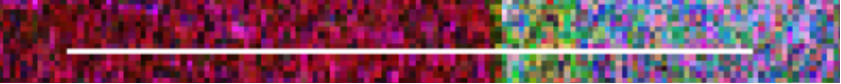
\includegraphics[width=13cm]{figures/single_data.pdf}};
    \node[above=-1pt of figure2] {Thin data strip};
    \node[below=-1pt of figure2] {$\bm z = (\underbrace{z_1,z_2,\dots,z_j}_{\bm z_\text{I}},\underbrace{z_{j+1}, z_{j+2},\dots,z_n}_{\bm z_\text{E}})$};
    \draw[-stealth, blue, line width=3pt] (text) -- (text1.north);
    \draw[-stealth, blue, line width=3pt] (text) -- (text2.north);
    \draw[-stealth, blue, line width=3pt] (text1.south) -- (text4.north);

	\draw[-stealth, blue, line width=3pt] (text4.south) to[out=-60,in=-120, looseness=1.2] node[midway, below, sloped, text=red] {\textbf{Maximum likelihood}} (text2.south);
	 % 
    \draw[-stealth, blue, line width=3pt] (text2.east) -- ++(1,0) -- ++(0,30) -- ++(2,0);		
  \end{tikzpicture}
\end{figure} 



\end{block}


%----------------------------------------------------------------------------------------

%----------------------------------------------------------------------------------------


\end{column} % End of the first column


\begin{column}{\sepwid}\end{column} % Empty spacer column


%----------------------------------------------------------------------------------------



\begin{column}{\onecolwid} % The second column
%----------------------------------------------------------------------------------------
%	The second column
%----------------------------------------------------------------------------------------

\begin{block}{\LARGE{EVIDENCES}}
\vspace{0.7em}

\begin{figure}[hbt]
%\label{fig:1}

  %\caption*{Intensity channels}
	\captionsetup[subfigure]{labelformat=empty}
    \begin{subfigure}{0.32\linewidth}
		    \centering
    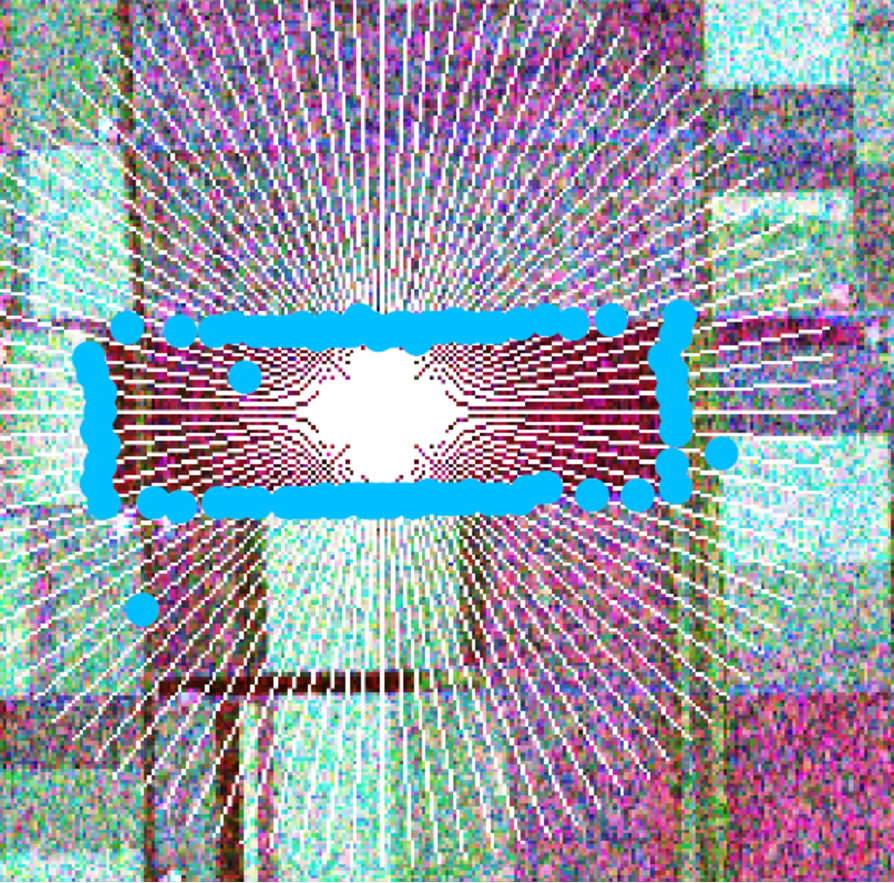
\includegraphics[width=\linewidth]{figures/hh_f.pdf}
    \caption{\large{Channel HH}}
    %\label{subfig:1ed}
  \end{subfigure}
  \begin{subfigure}{0.32\linewidth}
    \centering
    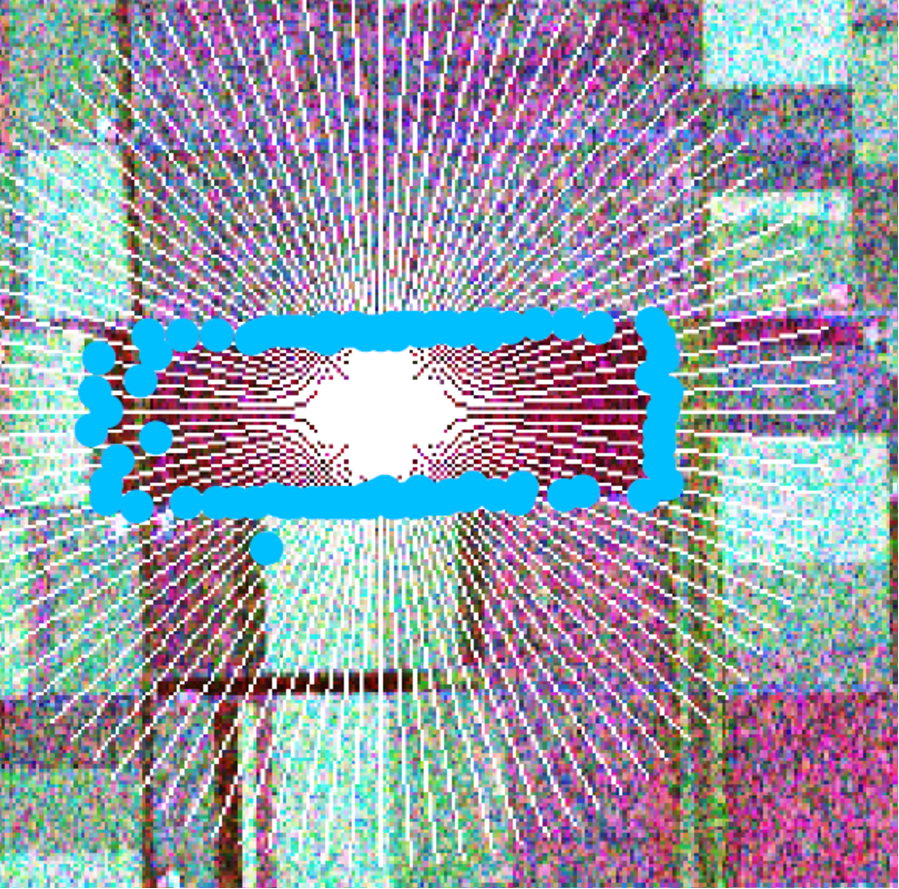
\includegraphics[width=\linewidth]{figures/hv.pdf}
    \caption{\large{Channel HV}}
    %\label{subfig:2ed}
  \end{subfigure}
  \begin{subfigure}{0.32\linewidth}
    \centering
    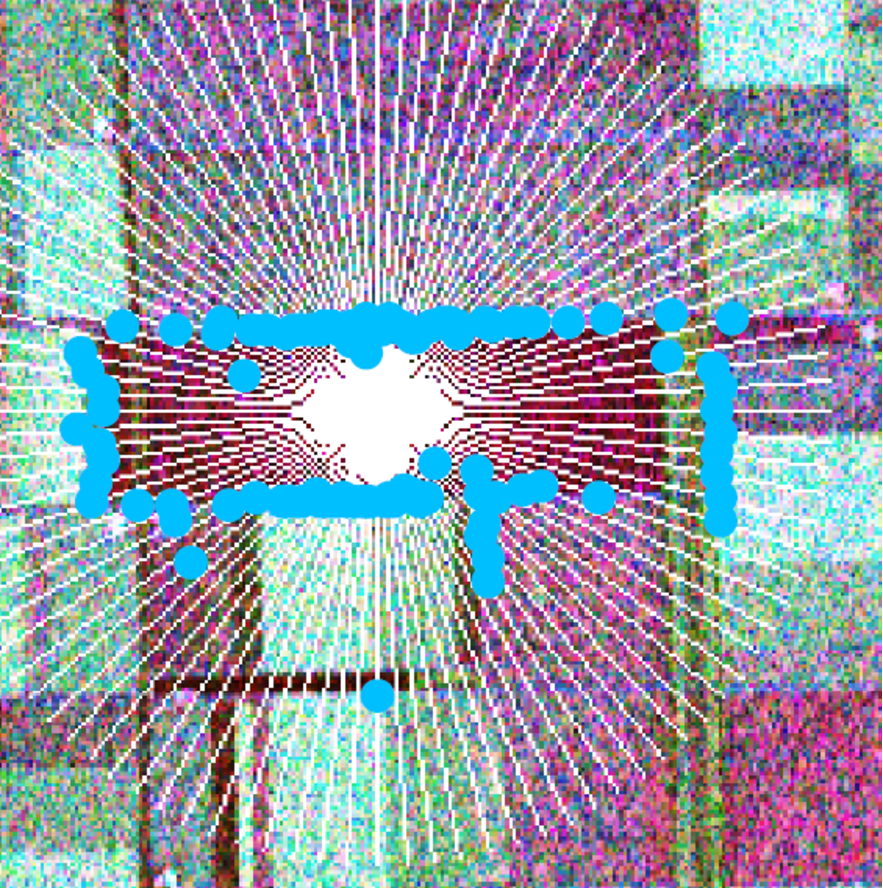
\includegraphics[width=\linewidth]{figures/vv_c.pdf}
    \caption{\large{Channel VV}}
    %\label{subfig:3ed}
  \end{subfigure}

\end{figure}
\vspace{-1.2cm}

	%-------------------------------------------------------------
\begin{figure}[h]
  \centering
  \begin{tikzpicture}
    \draw[double -stealth=10pt colored by blue!50!black and white] (0,0) -- (0,-2cm);
    \node[below] at (0,-2.5cm) {\textbf{\textcolor{blue!80!black}{\large{Fusion results}}}};
  \end{tikzpicture}
  % \caption{Figure}
\end{figure}
%-------------------------------------------------------------
\begin{figure}[hbt]
 %\caption*{Fusion methods.}
\captionsetup[subfigure]{labelformat=empty}
    \begin{subfigure}{0.32\linewidth}
    \centering
    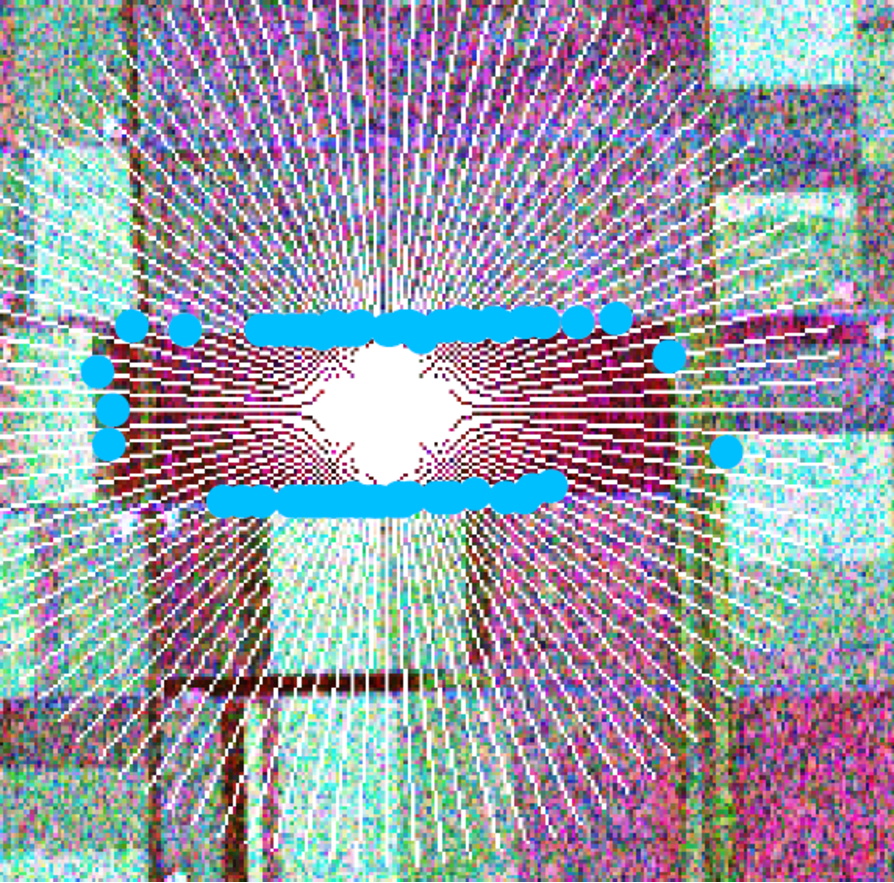
\includegraphics[width=\linewidth]{figures/roc.pdf}
    \caption{\large{S-ROC fusion}}
    %\label{subfig:1fus}
  \end{subfigure}
  \begin{subfigure}{0.33\linewidth}
    \centering
    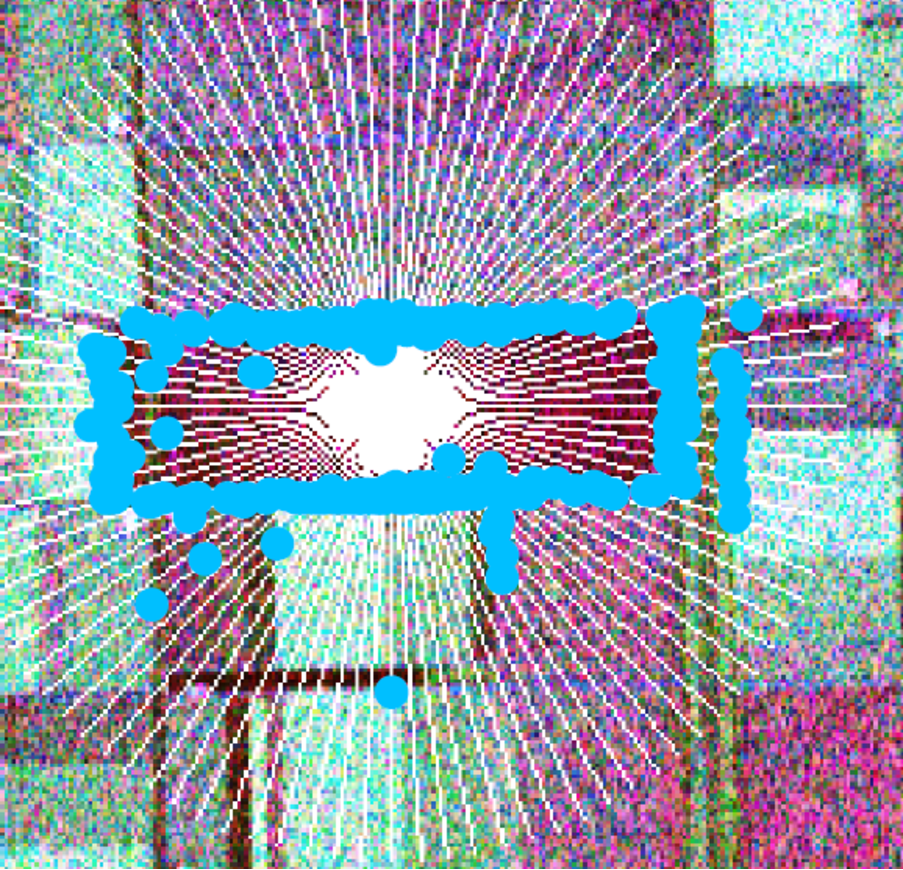
\includegraphics[width=\linewidth]{figures/pca_1.pdf}
    \caption{\large{PCA fusion}}
    %\label{subfig:2fus}
  \end{subfigure}
  \begin{subfigure}{0.32\linewidth}
    \centering
    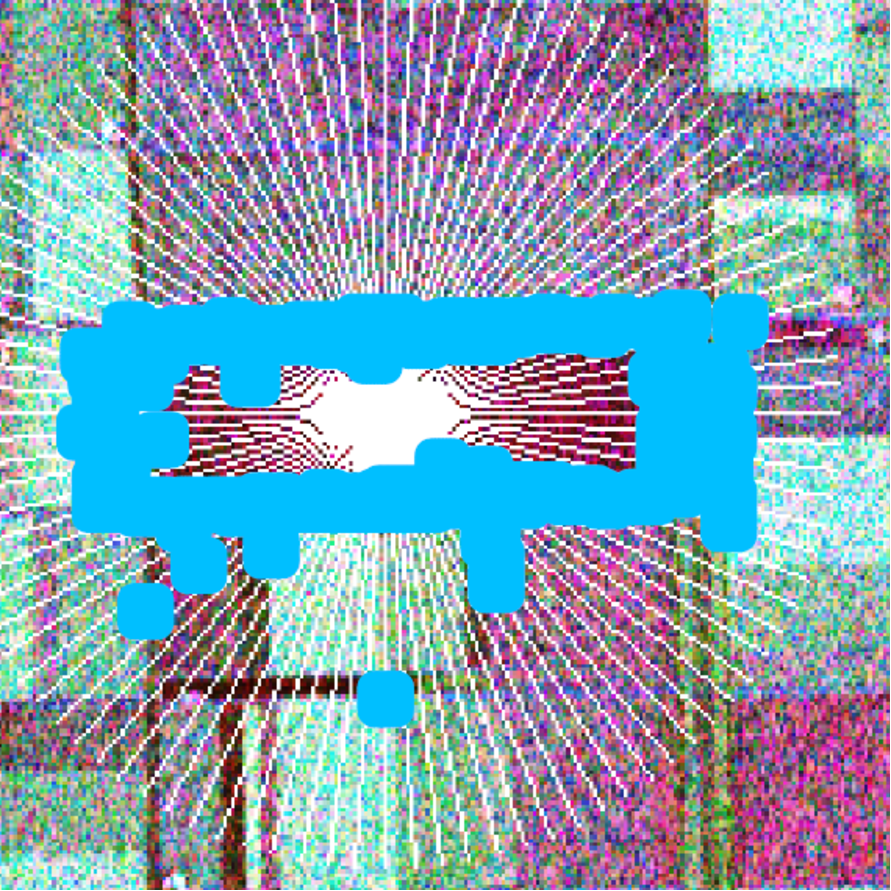
\includegraphics[width=\linewidth]{figures/swt.pdf}
    \caption{\large{MR-SWT fusion}}
   % \label{subfig:3fus}
  \end{subfigure}
  %\label{fig:1}
  \end{figure}
	
	%-------------------------------------------------------------
	\begin{figure}[h]
  \centering
  \begin{tikzpicture}
    \node[below=of text1, yshift=-1.5cm] (text4) {
      \begin{tcolorbox}[colback=blue!10,colframe=blue!30!black, arc=2pt, outer arc=2pt, nobeforeafter, width=16cm, center upper]
        \textcolor{blue}{\large{\textbf{{Shannon Entropy}}}}
				 \begin{equation*} 
         H(X)=-\sum_{i=1}^{n}p(x_i)\log_2p(x_i)
        \end{equation*}
      \end{tcolorbox}
    };
  \end{tikzpicture}
\end{figure}

	%-------------------------------------------------------------
	
	\begin{figure}[H]
	\captionsetup[subfigure]{labelformat=empty}
\captionsetup[subfigure]{justification=centering}
   \centering
    \begin{subfigure}{0.48\linewidth}
    %\centering
    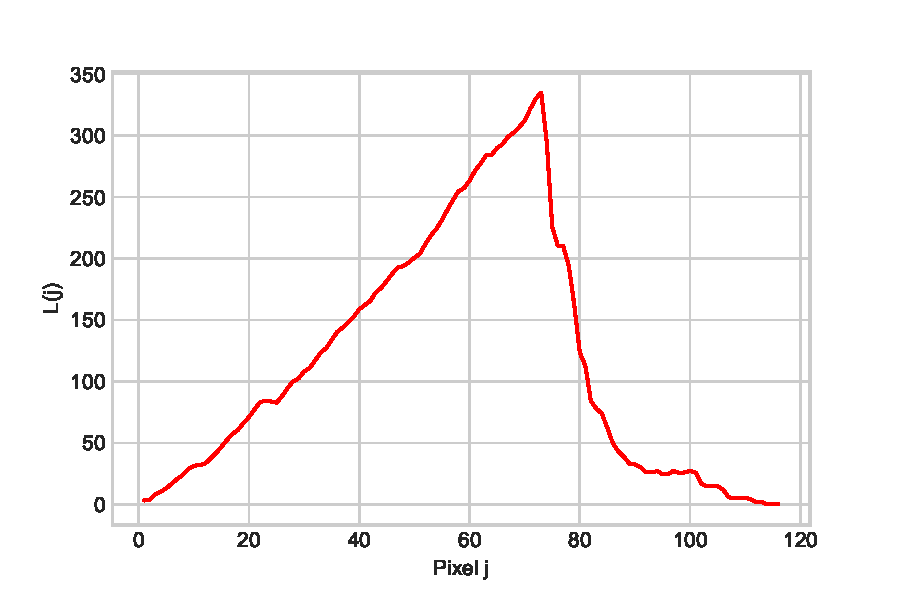
\includegraphics[width=17cm]{figures/likelihood_hh.pdf}
    \caption{\small{Channel HH (\textbf{Entropy = 0.0546}).}}
    %\label{subfig:1en}
  \end{subfigure}
  %\begin{subfigure}{0.49\linewidth}
   %% \centering
    %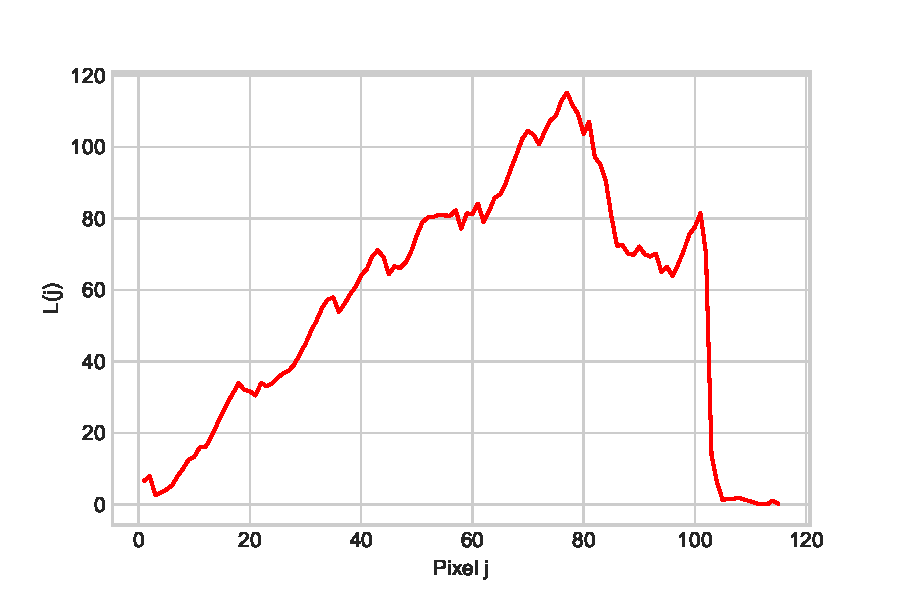
\includegraphics[width=4.2cm]{../figures/likelihood_hv.pdf}
 %\caption{\scriptsize{Channel HV (\textbf{Entropy =  0.6361}).}}
    %\label{subfig:2en}
  %\end{subfigure}\\
   \begin{subfigure}{0.48\linewidth}
    %\centering
    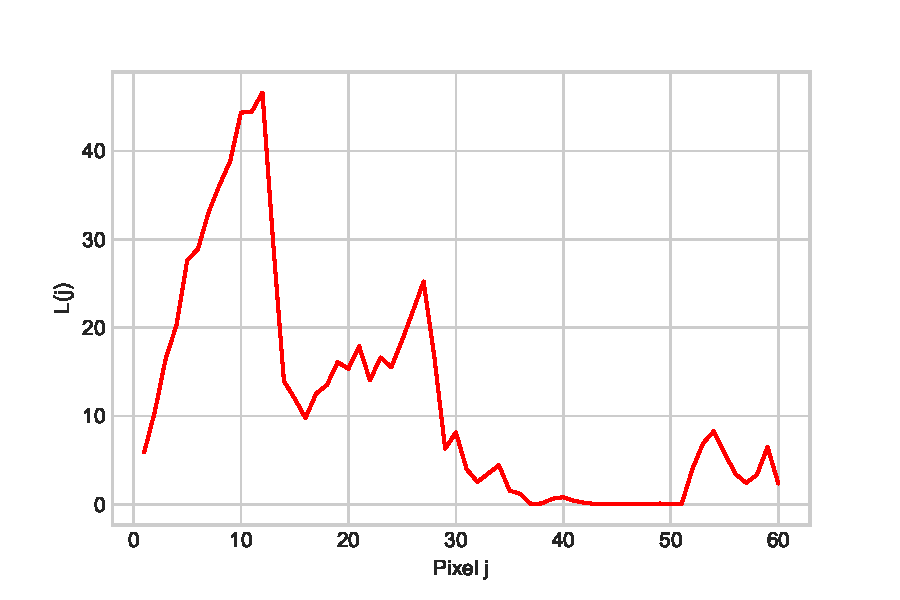
\includegraphics[width=17cm]{figures/likelihood_vv.pdf}
   % \centering
   \caption{\small{Channel VV (\textbf{Entropy = 0.8577}).}}
   % \label{subfig:3en}
  \end{subfigure}
 \end{figure}
	

\end{block}

\end{column} % End of column 2
%----------------------------------------------------------------------------------------


\begin{column}{\sepwid}\end{column} % Empty spacer column
%----------------------------------------------------------------------------------------
%	The third column
%----------------------------------------------------------------------------------------

\begin{column}{\onecolwid} % The third column

\begin{block}{\LARGE{ASSESSMENT}}
\vspace{0.7em}
\begin{table}[hbt]
  \centering
  \colorbox{violet!10}{%
 	\resizebox{0.7\textwidth}{!}{%
  \renewcommand{\arraystretch}{1.3}
  \begin{tabular}{@{}>{\bfseries}p{5.5cm}cccccc@{}}
	    \toprule
  
    \textcolor{blue!60}{\textbf{Method}}  & \textcolor{blue!60}{\textbf{Entropy}} & \textcolor{blue!60}{\textbf{MAE}}
		& \textcolor{blue!60}{\textbf{RMSE}} & \textcolor{blue!60}{\textbf{SD}} & \textcolor{blue!60}{\textbf{CC}} \\
    \midrule
    \textbf{HH}  & 6.6439      & 1.8400       & 3.7175   & 2.6291   & 0.9986 \\
    \textbf{HV}  & 6.6293      & 1.6700       & 2.9275   & 2.0640   & 0.9992 \\
    \textbf{VV}  & 6.6438      & 4.2400      & 7.9461    & 5.5649   & 0.9941 \\
    \textbf{S-ROC} & \textcolor{red}{6.0223}      & 1.4154      & 2.3664    & 1.6311    & \textcolor{red}{0.9994} \\
    \textbf{PCA} & 7.7944      & 3.0180       & 6.0657   & 4.2788  & 0.9964 \\
    \textbf{SWT} & 12.0914     & 5.8006      & 9.2486   & 6.4161  & 0.9932 \\
    \bottomrule
  \end{tabular}}}
\end{table}
\begin{figure}[h]
  \centering
  \begin{tikzpicture}
    \draw[double -stealth=10pt colored by blue!50!black and white] (0,0) -- (0,-2cm);
     \end{tikzpicture}
  % \caption{Figure}
\end{figure}

\vspace{-0.8cm}
\begin{figure}[h]
  \centering
  \begin{tikzpicture}
    \node[anchor=south west, inner sep=0] (image) at (0,0) {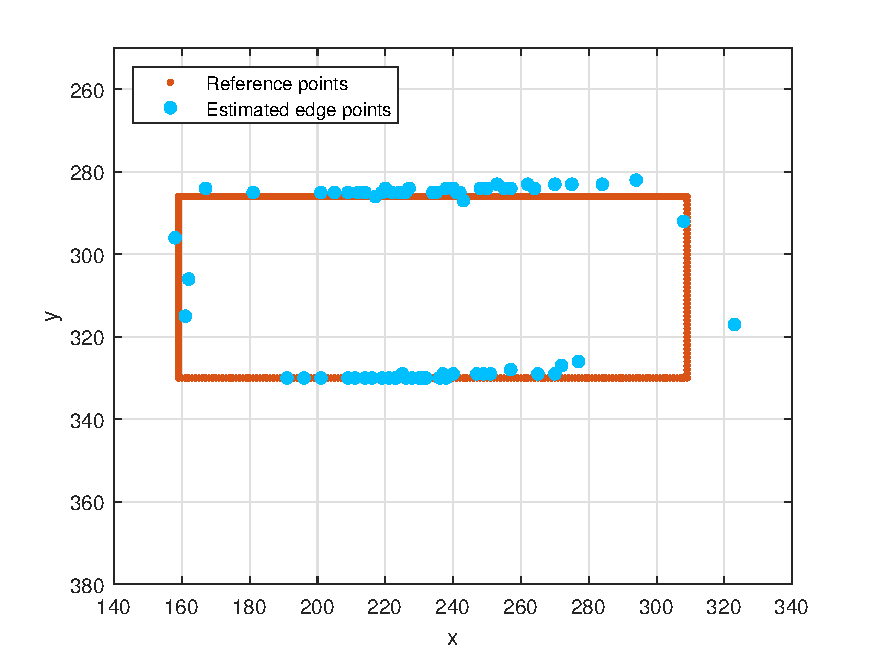
\includegraphics[width=29cm,height=17cm]{figures/roc_f.pdf}};
    \begin{scope}[x={(image.south east)},y={(image.north west)}]
      \node[above right, font=\bfseries\small, blue] at (0.4,0.1) {S-ROC Method};
    \end{scope}
  \end{tikzpicture}\vspace{-0.5cm}
  \caption*{\large{Estimated points vs. ground reference}}
\end{figure}
\vspace{-1.2cm}

\begin{figure}[H] 
\centering
	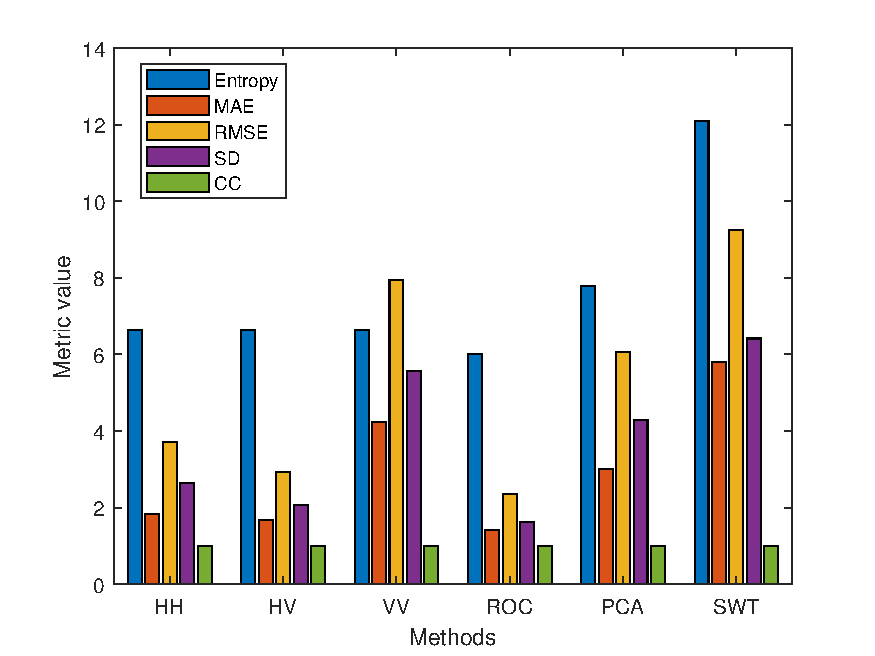
\includegraphics[width=29cm,height=17cm]{figures/metricas.pdf}
	%\caption*{\large{Quality metrics}}
	%\label{F5}
\end{figure}

\end{block}





%----------------------------------------------------------------------------------------
%	ACKNOWLEDGEMENTS
%----------------------------------------------------------------------------------------

%\setbeamercolor{block title}{fg=norange,bg=white} % Change the block title color
%
%\begin{block}{Acknowledgements}
	%
%
	%
%\end{block}

%----------------------------------------------------------------------------------------
%	CONTACT INFORMATION
%----------------------------------------------------------------------------------------


%\begin{block}{References}
%
	%{\footnotesize\bibliographystyle{abbrv} 
	%\bibliography{poster}}
%\end{block}


%----------------------------------------------------------------------------------------



\end{column} % End of the third column

\end{columns} % End of all the columns in the poster

\end{frame} % End of the enclosing frame

\end{document}
\begin{column}{\sepwid}\end{column} % Empty spacer column
